\begin{figure}[H]
\centering
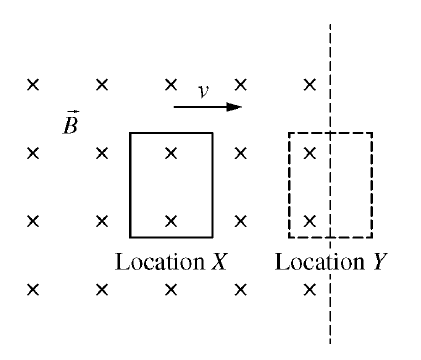
\includegraphics[scale=0.7]{images/22.png}
\end{figure}

% Multiple Choice Question 22
\begin{questions}\setcounter{question}{21}\question
A loop of wire at location $X$ is moving toward the right with constant speed $v$ in a region of uniform magnetic field $\vec{B}$, which is perpendicular to the plane of the loop. The magnetic field region ends at the dashed line, as shown in the figure above. Later, the loop is at location $Y$ and exiting the magnetic field with the same constant speed $v$. The process is then repeated with the loop moving at a speed of $2 v$. Which of the following best describes the emf in the loop at the two positions shown when the process is repeated at a speed of $2 v$ ?

\tabto{0.75cm}\underline{Emf at Location $X$}
\tabto{5.00cm}\underline{Emf at Location $Y$}

\begin{choices}
\choice Nonzero and halved  \tabto{4.25cm} Nonzero and halved
\choice Nonzero and doubled \tabto{4.25cm} Nonzero and doubled
\choice Nonzero and doubled \tabto{4.25cm} Zero at both speeds
\choice Zero at both speeds \tabto{4.25cm} Zero at both speeds
\choice Zero at both speeds \tabto{4.25cm} Nonzero and doubled
\end{choices}\end{questions}
